\documentclass[conference]{IEEEtran}
\IEEEoverridecommandlockouts

\usepackage{cite}
\usepackage{amsmath,amssymb,amsfonts}
\usepackage{graphicx}
\usepackage{booktabs}
\usepackage{array}
\usepackage{xcolor}
\usepackage{url}
\usepackage{tikz}
\usetikzlibrary{arrows.meta,positioning,shapes.geometric}
\usepackage[hidelinks]{hyperref}

\graphicspath{{figures/}}

\begin{document}

\title{Auditing and Revalidating a Machine-Learning Diabetes
Prediction System: A Case Study on Data Leakage and Clinical Deployment}

\author{\IEEEauthorblockN{PREDIA Research Group}
\IEEEauthorblockA{\textit{Clinical Informatics and Applied Machine Learning} \\
\textit{PREDIA Project} \\
M\'exico \\
predia@example.org}}

\maketitle

\begin{abstract}
Machine-learning systems are increasingly embedded in clinical software, yet
their reported performance is often accepted without methodological scrutiny.
We report an audit of the diabetes-prediction module of PREDIA, a production
electronic health-record platform whose model advertised a 97.89\% accuracy.
Working exclusively from the project's own artifacts, we show that this figure
is neither reproducible nor honest: the deployed estimator is a logistic
regression hardcoded in TypeScript, trained on a different 947-sample dataset
whose features (urea, creatinine, VLDL) are absent from the platform's
100{,}000-row corpus, and its accuracy is inflated by \emph{target leakage}
through HbA1c, an official diagnostic criterion for diabetes. A five-fold
cross-validated probe confirms that HbA1c alone attains 0.93 ROC-AUC, whereas a
leakage-free \emph{screening} model reaches only $\approx$0.66. We retrain and
compare nine classifiers under a leakage-controlled protocol with stratified
cross-validation and a clinically oriented metric panel; logistic regression is
the best honest model (ROC-AUC 0.659, MCC 0.223). We interpret it with
permutation importance and SHAP, and migrate it into the PREDIA REST API as a
self-contained TypeScript model with a redesigned, leakage-free feature
contract. The study contributes a reproducible audit methodology and a candid
account of the gap between inflated and honest metrics in clinical ML.
\end{abstract}

\begin{IEEEkeywords}
data leakage, diabetes prediction, model auditing, reproducibility,
clinical decision support, interpretability, machine learning
\end{IEEEkeywords}

\section{Introduction}
Diabetes mellitus is a leading global public-health burden, affecting an
estimated 537 million adults worldwide~\cite{idf2021atlas}. Because early
identification of at-risk individuals enables preventive intervention, machine
learning (ML) has been widely proposed for diabetes risk stratification.
However, the clinical value of such models depends entirely on the
\emph{validity} of their reported performance. When a model is evaluated
incorrectly---most commonly through \emph{data leakage}, the inadvertent use of
information unavailable at prediction time or that encodes the
outcome---reported metrics become severely inflated and the system fails
silently in deployment~\cite{kaufman2012leakage,kapoor2023leakage}.

This paper is a case study of exactly such a failure, discovered while auditing
PREDIA, a production electronic health-record (EHR) platform. PREDIA shipped a
diabetes-prediction module advertising a 97.89\% accuracy. Rather than accept
this number, we subjected the model and its data to a reproducible audit using
only the project's own artifacts.

\textbf{Objectives.} (i)~Determine whether PREDIA's reported accuracy is valid
and reproducible; (ii)~test for data leakage and methodological flaws;
(iii)~establish an honest performance baseline by retraining and comparing
multiple classifiers under a leakage-controlled protocol; and (iv)~deploy the
selected model back into PREDIA without breaking the platform.

\textbf{Contributions.} (1)~A formal, reproducible audit demonstrating that the
deployed model's accuracy is both irreproducible (trained on a different dataset
with absent features) and inflated by HbA1c leakage. (2)~A leakage-controlled
benchmark of nine classifiers, separating an honest \emph{screening} framing
from a \emph{clinical} framing that quantifies the leakage contribution
($+0.285$ ROC-AUC). (3)~Interpretability and clinical analysis of the honest
model. (4)~A production migration of the revalidated model into the PREDIA REST
API with a redesigned, leakage-free feature contract.

\section{Related Work}
Tree- and kernel-based learners dominate tabular clinical prediction: random
forests~\cite{breiman2001random}, gradient-boosted trees as implemented in
XGBoost~\cite{chen2016xgboost} and LightGBM~\cite{ke2017lightgbm}, support-vector
machines~\cite{cortes1995svm}, and nearest-neighbour
classifiers~\cite{cover1967knn}. All experiments here use the
\texttt{scikit-learn} ecosystem~\cite{pedregosa2011scikit}. For model
interpretability we adopt SHAP values~\cite{lundberg2017shap} alongside
permutation importance~\cite{breiman2001random}.

Data leakage is a long-recognised but persistent threat to the validity of ML
studies~\cite{kaufman2012leakage}; recent work documents it as a primary driver
of the reproducibility crisis in ML-based science across
disciplines~\cite{kapoor2023leakage}. In clinical contexts, leakage frequently
arises from including diagnostic measurements that \emph{define} the label. The
diagnosis of diabetes is governed by laboratory thresholds---HbA1c
$\geq 6.5\%$ being a primary criterion~\cite{ada2021classification}---so any
model that consumes HbA1c to predict a HbA1c-derived label is, by construction,
leaking. Because accuracy is misleading under class imbalance, we report the
Matthews correlation coefficient (MCC), which is more informative for binary
classification~\cite{chicco2020mcc}. Finally, the original PREDIA model was
trained on a small public diabetes dataset~\cite{rashid2020diabetes} whose
feature set differs from the platform's operational data---a discrepancy central
to our findings.

\section{Methodology}
\subsection{Dataset}
All experiments use \texttt{diabetes\_dataset.csv}, the corpus shipped with the
PREDIA repository (Table~\ref{tab:dataset}). It contains 100{,}000 instances and
31 attributes describing demographics, socio-economic status, lifestyle,
anthropometry, vital signs, lipid profile and laboratory measurements. The
binary target \texttt{diagnosed\_diabetes} is mildly imbalanced (60.0\% positive
/ 40.0\% negative, ratio 1.50). The corpus has no missing values and no
duplicated rows.

\begin{table}[!t]
\renewcommand{\arraystretch}{1.2}
\caption{Characteristics of the \texttt{diabetes\_dataset.csv} corpus}
\label{tab:dataset}
\centering
\begin{tabular}{l l}
\toprule
\textbf{Property} & \textbf{Value} \\
\midrule
Instances & 100{,}000 \\
Total columns & 31 \\
Numeric attributes & 24 (incl.\ target) \\
Categorical attributes & 7 \\
Target variable & \texttt{diagnosed\_diabetes} \\
Positive class (Diabetes) & 59{,}998 (60.0\%) \\
Negative class (No Diabetes) & 40{,}002 (40.0\%) \\
Imbalance ratio & 1.50 \\
Missing values & 0 \\
Duplicated rows & 0 \\
Train/test split & 80{,}000 / 20{,}000 (stratified) \\
\bottomrule
\end{tabular}
\end{table}


\subsection{Leakage-aware feature taxonomy}
The defining methodological decision of this study is an explicit feature
taxonomy that controls leakage:
\begin{itemize}
\item \textbf{Direct leakage (always removed):} \texttt{diabetes\_stage} (the
diagnostic category itself) and \texttt{diabetes\_risk\_score} (a derived
risk proxy).
\item \textbf{Diagnostic laboratories:} \texttt{hba1c},
\texttt{glucose\_fasting}, \texttt{glucose\_postprandial} and
\texttt{insulin\_level}. Being diagnostic criteria, they are \emph{excluded}
from the honest \emph{screening} framing and \emph{included} only in a
\emph{clinical} framing used to quantify their (leaking) contribution.
\item \textbf{Screening features:} demographics, socio-economic status,
lifestyle, family history, anthropometry, vital signs and lipid profile---the
24 inputs that a pre-diagnostic risk tool can legitimately collect.
\end{itemize}
Fig.~\ref{fig:leakcorr} confirms that the variables most correlated with the
target are precisely the diagnostic laboratories, motivating this separation.

\begin{figure}[!t]
\centering
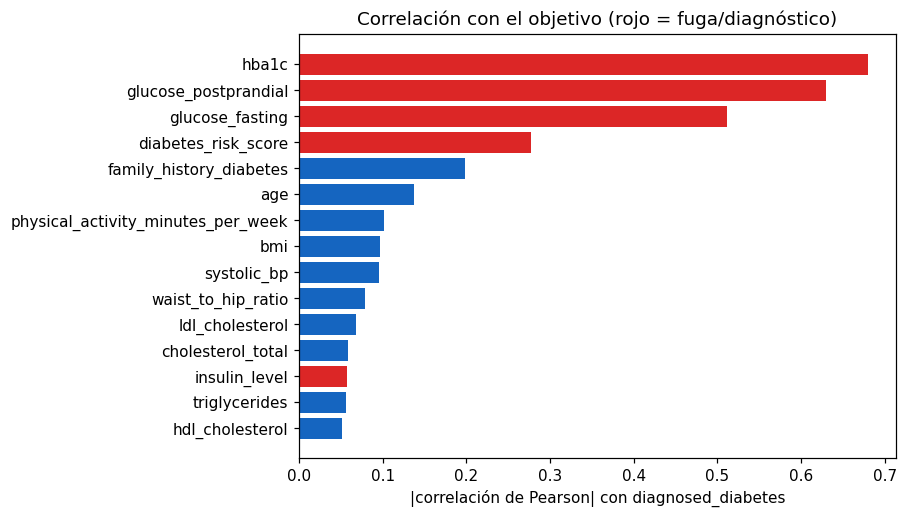
\includegraphics[width=\columnwidth]{leakage_correlation.png}
\caption{Absolute Pearson correlation with the target. The strongest signals
(red) are diagnostic/leaky variables (\texttt{hba1c}, \texttt{glucose\_*},
\texttt{diabetes\_risk\_score}); legitimate screening variables (blue) are
weakly correlated.}
\label{fig:leakcorr}
\end{figure}

\subsection{Preprocessing, validation and pipeline}
Categorical attributes are one-hot encoded and numeric attributes standardised
($z$-score); binary attributes pass through. All transformations are fitted
\emph{inside} a \texttt{scikit-learn} \texttt{Pipeline}~\cite{pedregosa2011scikit}
to prevent train/test contamination. We use an 80/20 stratified split and
4-fold stratified cross-validation for model selection, with a global random
seed of 42 for full reproducibility. Fig.~\ref{fig:pipeline} summarises the
end-to-end protocol.

\begin{figure}[!t]
\centering
\resizebox{0.95\columnwidth}{!}{%
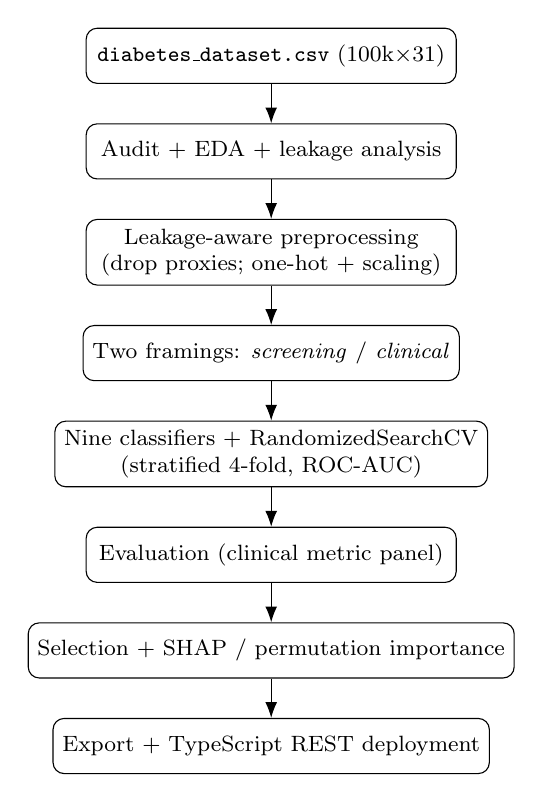
\begin{tikzpicture}[
  node distance=5mm,
  box/.style={draw, rounded corners, align=center, font=\footnotesize,
              minimum width=4.7cm, minimum height=7mm},
  arr/.style={-{Latex[length=2mm]}}]
\node[box] (data) {\texttt{diabetes\_dataset.csv} (100k$\times$31)};
\node[box, below=of data] (audit) {Audit + EDA + leakage analysis};
\node[box, below=of audit] (prep) {Leakage-aware preprocessing\\(drop proxies; one-hot + scaling)};
\node[box, below=of prep] (fram) {Two framings: \emph{screening} / \emph{clinical}};
\node[box, below=of fram] (zoo) {Nine classifiers + RandomizedSearchCV\\(stratified 4-fold, ROC-AUC)};
\node[box, below=of zoo] (eval) {Evaluation (clinical metric panel)};
\node[box, below=of eval] (sel) {Selection + SHAP / permutation importance};
\node[box, below=of sel] (dep) {Export + TypeScript REST deployment};
\foreach \a/\b in {data/audit,audit/prep,prep/fram,fram/zoo,zoo/eval,eval/sel,sel/dep}
  \draw[arr] (\a) -- (\b);
\end{tikzpicture}}
\caption{Reproducible audit-to-deployment pipeline.}
\label{fig:pipeline}
\end{figure}

\section{Audit of the Original Model}
\subsection{Architecture and reported performance}
Inspection of the serialized artifact (\texttt{modelo\_diabetes.pkl}) shows the
deployed estimator is a \emph{logistic regression} with 11 input features
(\texttt{Gender, AGE, Urea, Cr, HbA1c, Chol, TG, HDL, LDL, VLDL, BMI}), a single
intercept of $7.578$, trained on 947 samples (757 train / 190 test). The
platform metadata and database seed report an accuracy of $0.9789$, while the
in-code documentation simultaneously states $98.42\%$ accuracy, $100\%$
precision and $0.9975$ AUC---an internal inconsistency that already undermines
confidence.

\subsection{Reproducibility and dataset/feature mismatch}
No training code or notebook exists in the repository; the methodology is
therefore not reproducible. Moreover, the deployed model was trained on a
different corpus (the 947-sample public dataset~\cite{rashid2020diabetes}):
three of its eleven features---\texttt{Urea}, \texttt{Cr} and \texttt{VLDL}---are
\emph{absent} from PREDIA's operational dataset, and the lipid features use an
incompatible unit scale. The model cannot be evaluated as-is on the platform's
own data. We further observe that, at serving time, the model is not loaded from
the \texttt{.pkl} file at all but reimplemented as hardcoded coefficients in
TypeScript, augmented by hand-written clinical override rules.

\subsection{Data leakage}
HbA1c is the second most important feature of the original model, yet
HbA1c $\geq 6.5\%$ \emph{is} the diagnostic criterion for
diabetes~\cite{ada2021classification}. Using it as a predictor therefore leaks
the label. Table~\ref{tab:leakage} quantifies this with five-fold
cross-validated logistic regressions on isolated feature subsets: HbA1c alone
already yields 0.93 ROC-AUC, the pure-proxy pair
\texttt{diabetes\_stage}+\texttt{risk\_score} reaches 0.997, whereas a
leakage-free screening subset attains only 0.61. The reported $\approx$98\%
accuracy is thus only attainable with diagnostic/leaking variables; it reflects
leakage, not pre-diagnostic predictive skill.

\begin{table}[!t]
\renewcommand{\arraystretch}{1.2}
\caption{Leakage demonstration: 5-fold cross-validated logistic regression
trained on isolated feature subsets of \texttt{diabetes\_dataset.csv}}
\label{tab:leakage}
\centering
\begin{tabular}{l c c}
\toprule
\textbf{Feature subset} & \textbf{Accuracy} & \textbf{ROC-AUC} \\
\midrule
\texttt{hba1c} only & 0.8520 & 0.9325 \\
\texttt{glucose\_fasting} only & 0.7307 & 0.8082 \\
Diagnostic labs (HbA1c+glucose+insulin) & 0.8567 & 0.9337 \\
\texttt{diabetes\_stage}+\texttt{risk\_score} & \textbf{0.9979} & \textbf{0.9974} \\
\midrule
Screening (non-diagnostic numeric) & 0.6163 & 0.6121 \\
\bottomrule
\end{tabular}
\end{table}


\section{Experimentation}
We retrained nine classifiers under the screening framing:
logistic regression, random forest~\cite{breiman2001random}, extra trees,
histogram gradient boosting, XGBoost~\cite{chen2016xgboost},
LightGBM~\cite{ke2017lightgbm}, support-vector machine (RBF
kernel)~\cite{cortes1995svm}, $k$-nearest neighbours~\cite{cover1967knn} and a
multilayer perceptron. Each estimator is wrapped in the common preprocessing
pipeline and tuned with \texttt{RandomizedSearchCV} (8 candidates,
stratified 4-fold, scoring ROC-AUC). Because the kernel SVM and KNN scale poorly
to $8\times10^4$ training rows, they are tuned on an 8{,}000-row stratified
subsample and evaluated on the full test set; this is reported explicitly. All
runs share \texttt{random\_state}=42.

\section{Results}
Table~\ref{tab:comparison} reports the test-set performance of all nine models
under the honest screening framing. Three findings stand out. First, the honest
problem is genuinely hard: every model clusters around ROC-AUC $0.65$--$0.66$.
Second, \emph{logistic regression is the best honest model} by ROC-AUC
($0.6591$) and by MCC ($0.2229$), and is also the best calibrated and most
balanced. Third, the tree ensembles and SVM trade specificity for sensitivity
(e.g.\ SVM reaches $0.96$ sensitivity but $0.09$ specificity), which inflates F1
without improving discrimination. The comparative ROC and ROC-AUC summaries are
shown in Figs.~\ref{fig:roc} and~\ref{fig:auc}; the confusion matrix and
reliability diagram of the selected model appear in Figs.~\ref{fig:cm}
and~\ref{fig:cal}.

\begin{table*}[!t]
\renewcommand{\arraystretch}{1.25}
\caption{Test-set performance of nine classifiers under the honest \emph{screening}
framing (no diagnostic laboratory features). Models sorted by ROC-AUC. Best value
per column in bold. $\dagger$ tuned on an 8{,}000-row stratified subsample.}
\label{tab:comparison}
\centering
\begin{tabular}{l c c c c c c c c c}
\toprule
\textbf{Model} & \textbf{Acc.} & \textbf{Bal.\,Acc.} & \textbf{Prec.} & \textbf{Sens.} & \textbf{Spec.} & \textbf{F1} & \textbf{ROC-AUC} & \textbf{MCC} & \textbf{CV-AUC} \\
\midrule
Logistic Regression      & 0.6044 & \textbf{0.6136} & \textbf{0.7144} & 0.5675 & \textbf{0.6597} & 0.6325 & \textbf{0.6591} & \textbf{0.2229} & \textbf{0.6610} \\
Hist.\ Gradient Boosting & \textbf{0.6310} & 0.5790 & 0.6489 & 0.8391 & 0.3189 & 0.7318 & 0.6579 & 0.1856 & 0.6591 \\
XGBoost                  & 0.6289 & 0.5781 & 0.6488 & 0.8317 & 0.3246 & 0.7289 & 0.6573 & 0.1817 & 0.6587 \\
LightGBM                 & 0.6280 & 0.5753 & 0.6464 & 0.8387 & 0.3119 & 0.7301 & 0.6558 & 0.1776 & 0.6574 \\
Random Forest            & 0.6244 & 0.5594 & 0.6340 & 0.8848 & 0.2340 & 0.7387 & 0.6549 & 0.1576 & 0.6573 \\
Extra Trees              & 0.6194 & 0.5438 & 0.6237 & \textbf{0.9220} & 0.1656 & 0.7441 & 0.6538 & 0.1356 & 0.6551 \\
MLP (Neural Net)         & 0.6244 & 0.5821 & 0.6541 & 0.7937 & 0.3704 & 0.7172 & 0.6530 & 0.1807 & 0.6555 \\
SVM (RBF)$^{\dagger}$    & 0.6123 & 0.5254 & 0.6130 & 0.9600 & 0.0907 & \textbf{0.7482} & 0.6328 & 0.1044 & 0.6360 \\
KNN$^{\dagger}$          & 0.6003 & 0.5441 & 0.6268 & 0.8251 & 0.2631 & 0.7124 & 0.5845 & 0.1061 & 0.5872 \\
\bottomrule
\end{tabular}
\end{table*}


\begin{figure}[!t]
\centering
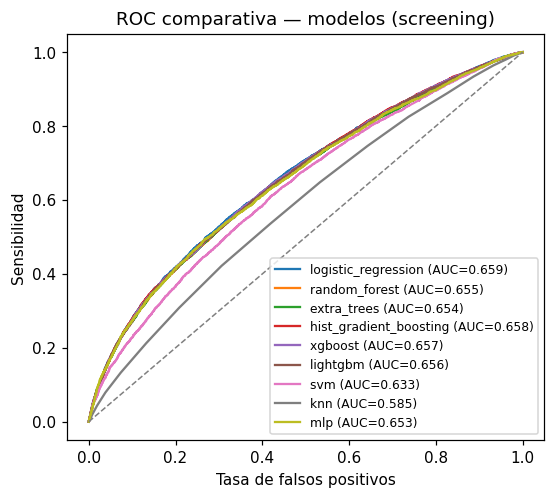
\includegraphics[width=\columnwidth]{comparison_roc.png}
\caption{Comparative ROC curves of the nine classifiers (screening framing).}
\label{fig:roc}
\end{figure}

\begin{figure}[!t]
\centering
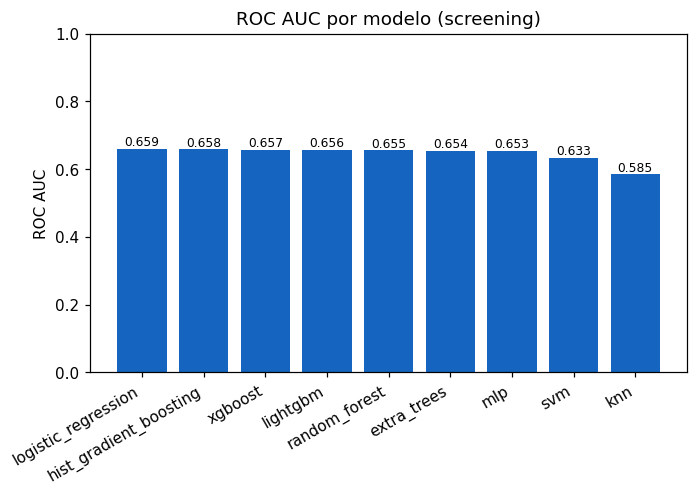
\includegraphics[width=\columnwidth]{comparison_auc.png}
\caption{ROC-AUC per model (screening framing).}
\label{fig:auc}
\end{figure}

\begin{figure}[!t]
\centering
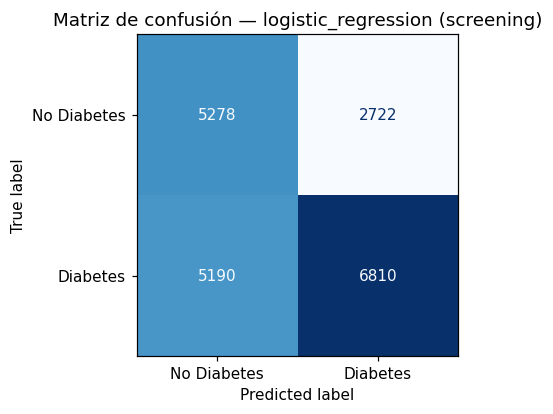
\includegraphics[width=0.78\columnwidth]{cm_screening_logistic_regression.png}
\caption{Confusion matrix of the selected logistic-regression screening model on
the 20{,}000-instance test set.}
\label{fig:cm}
\end{figure}

\begin{figure}[!t]
\centering
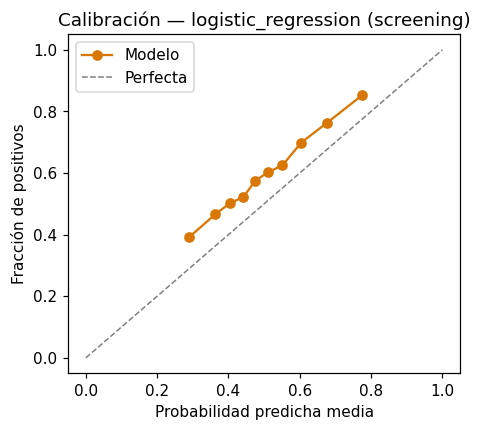
\includegraphics[width=0.82\columnwidth]{cal_screening_logistic_regression.png}
\caption{Reliability (calibration) diagram of the selected model.}
\label{fig:cal}
\end{figure}

To quantify the leakage contribution directly, Table~\ref{tab:framing} contrasts
the screening framing with a clinical framing that re-introduces the diagnostic
laboratories. Adding those features raises ROC-AUC from $\approx$0.66 to
$\approx$0.94---a mean increase of $+0.285$---confirming that the original
system's apparent excellence was almost entirely leakage.

\begin{table}[!t]
\renewcommand{\arraystretch}{1.2}
\caption{Effect of including diagnostic laboratory features: honest
\emph{screening} framing vs.\ \emph{clinical} framing (with HbA1c, glucose and
insulin). The ROC-AUC gap quantifies the contribution of information leakage.}
\label{tab:framing}
\centering
\begin{tabular}{l c c c c}
\toprule
& \multicolumn{2}{c}{\textbf{Screening}} & \multicolumn{2}{c}{\textbf{Clinical}} \\
\cmidrule(lr){2-3}\cmidrule(lr){4-5}
\textbf{Model} & Acc. & ROC-AUC & Acc. & ROC-AUC \\
\midrule
Logistic Regression & 0.6044 & 0.6591 & 0.8878 & 0.9339 \\
Random Forest       & 0.6244 & 0.6549 & 0.9196 & 0.9417 \\
XGBoost             & 0.6289 & 0.6573 & 0.9199 & 0.9444 \\
\midrule
\multicolumn{1}{l}{\textbf{Mean $\Delta$ ROC-AUC}} & \multicolumn{4}{c}{$+0.285$ (leakage contribution)} \\
\bottomrule
\end{tabular}
\end{table}


\section{Interpretability}
We interpret the selected model with permutation importance (drop in test
ROC-AUC) and SHAP values~\cite{lundberg2017shap}. Both methods agree closely
(Table~\ref{tab:importance}, Figs.~\ref{fig:perm} and~\ref{fig:shap}):
\texttt{family\_history\_diabetes}, \texttt{age} and
\texttt{physical\_activity\_minutes\_per\_week} dominate, followed by
\texttt{bmi} and \texttt{diet\_score}.

\begin{table}[!t]
\renewcommand{\arraystretch}{1.2}
\caption{Most influential features of the selected screening model, by
permutation importance (drop in ROC-AUC) and by mean absolute SHAP value.}
\label{tab:importance}
\centering
\begin{tabular}{l c | l c}
\toprule
\multicolumn{2}{c|}{\textbf{Permutation importance}} & \multicolumn{2}{c}{\textbf{SHAP (mean $|\phi|$)}} \\
Feature & $\Delta$AUC & Feature & $|\phi|$ \\
\midrule
family\_history\_diabetes & 0.0816 & age & 0.0539 \\
age & 0.0340 & family\_history\_diabetes & 0.0536 \\
physical\_activity & 0.0179 & physical\_activity & 0.0362 \\
bmi & 0.0037 & bmi & 0.0220 \\
diet\_score & 0.0023 & diet\_score & 0.0126 \\
hdl\_cholesterol & 0.0013 & hdl\_cholesterol & 0.0125 \\
screen\_time & 0.0012 & triglycerides & 0.0082 \\
triglycerides & 0.0008 & screen\_time & 0.0076 \\
\bottomrule
\end{tabular}
\end{table}


\begin{figure}[!t]
\centering

\includegraphics[width=\columnwidth]{permutation_importance.png}
\caption{Permutation importance of the selected screening model.}
\label{fig:perm}
\end{figure}

\begin{figure}[!t]
\centering
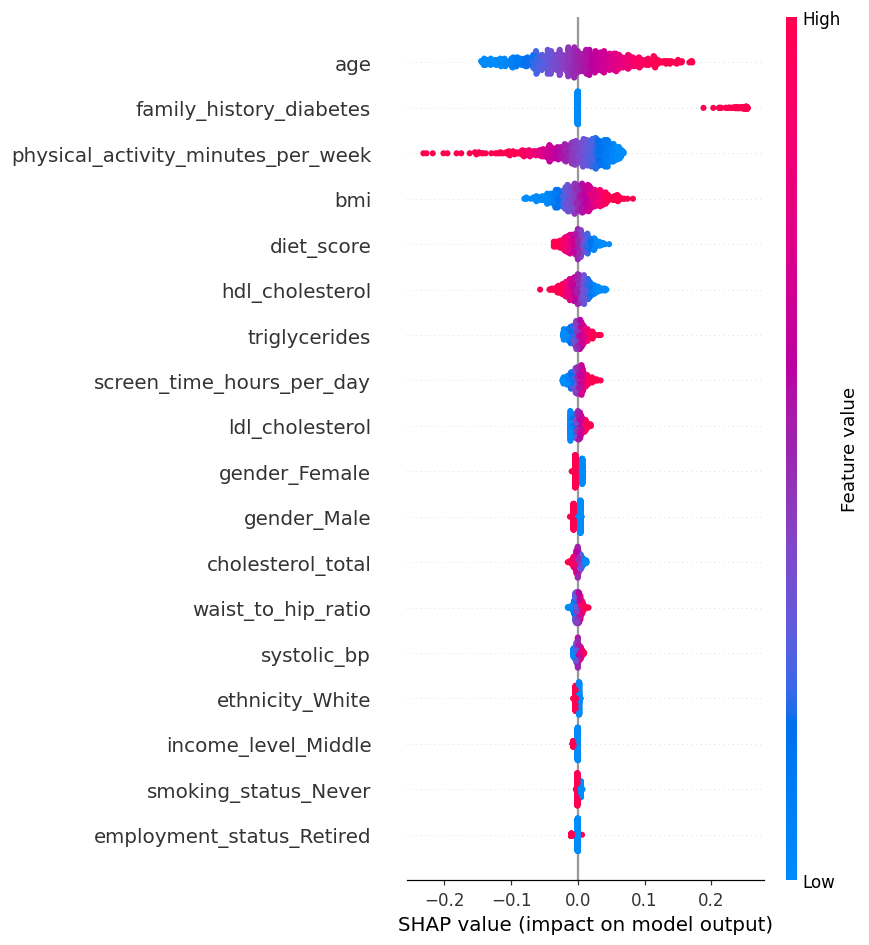
\includegraphics[width=\columnwidth]{shap_summary.png}
\caption{SHAP summary (beeswarm) of the selected screening model.}
\label{fig:shap}
\end{figure}

\textbf{Clinical impact.} Reassuringly, the dominant predictors are
\emph{modifiable or routinely recordable} without laboratory testing (family
history, physical activity, body-mass index, diet), which is exactly what a
pre-diagnostic screening tool should rely upon. \textbf{Risks of
interpretation.} Importance does not imply causation; the associations are
observational, the corpus is of unknown provenance, and the modest effect sizes
mean individual predictions carry substantial uncertainty.

\section{Discussion}
\textbf{Why the original model looked excellent.} Its $\approx$98\% accuracy was
the joint product of two artifacts: evaluation on a different, smaller dataset,
and target leakage through HbA1c. Neither reflects the model's ability to
anticipate diabetes before diagnosis.
\textbf{Inflated vs.\ honest metrics.} The same algorithm (logistic regression)
moves from ROC-AUC $0.93$ (with leakage) to $0.66$ (leakage-free); accuracy
under imbalance is especially misleading here, which is why we emphasise MCC and
balanced accuracy~\cite{chicco2020mcc}.
\textbf{Clinical implications.} An honest pre-diagnostic signal of ROC-AUC
$\approx$0.66 is modest; the model is defensible only as decision \emph{support}
and must never be presented as a diagnosis.
\textbf{Dataset limitations.} The corpus is synthetic-looking, of undocumented
provenance, lacks external validity, and bundles diagnosis-defining variables
that make naive modelling dangerous.
\textbf{Deployment risks.} Shipping a leakage-inflated model invites automation
bias and unsafe clinical reliance; this motivated both the revalidation and the
redesigned feature contract.

\section{Production Integration}
The revalidated model was integrated into PREDIA while preserving the platform's
constraints. (i)~\textbf{Architecture decision:} the serving runtime is
pure TypeScript (no Python sidecar), chosen for portability; we therefore
exported the logistic-regression screening model---which is also the best honest
model---as plain coefficients plus the one-hot/scaling parameters, consumed
generically at inference. (ii)~\textbf{Export:} the full
\texttt{scikit-learn} pipeline is serialized (\texttt{joblib}/\texttt{pickle})
for reproducibility, and a JSON parameter file is generated for the TypeScript
runtime. (iii)~\textbf{REST API:} the \texttt{/api/predicciones/nueva} endpoint
and its validation schema were migrated to the new 24-feature, leakage-free
contract; the web prediction form was rewritten accordingly. (iv)~\textbf{
Compatibility:} prediction \emph{reads} (e.g.\ the mobile application) were
unaffected, since only prediction \emph{creation} changed; reported model
metadata was corrected from the inflated 97.89\% to the honest value. An
end-to-end test confirmed the migrated endpoint returns coherent predictions.

\section{Conclusions}
We audited a production diabetes-prediction system and showed, using only the
project's own evidence, that its headline 97.89\% accuracy was neither
reproducible nor honest: it stemmed from a dataset/feature mismatch and from
HbA1c-mediated target leakage. A leakage-controlled re-benchmark of nine models
established an honest baseline (logistic regression, ROC-AUC $0.659$, MCC
$0.223$), which we interpreted and redeployed into PREDIA with a corrected
feature contract. The central lesson is methodological: in clinical ML,
near-perfect metrics are a warning sign, and disciplined leakage control,
reproducibility and honest reporting matter more than headline accuracy.

\section{Future Work}
Future directions include: collecting a larger, clinically labelled and
documented cohort; multicentric and temporal external validation; probability
calibration and threshold optimisation against clinical cost (favouring
sensitivity); subgroup fairness analysis across ethnicity and sex; privacy-
preserving \emph{federated learning} across institutions; and richer explainable
-AI tooling integrated into the clinician workflow.

\section*{Reproducibility}
All artifacts (executed notebooks, trained models, metrics, figures and reports)
are provided in the \texttt{ml-research/} directory with a pinned
\texttt{requirements.txt} and a global seed of 42.

\bibliographystyle{IEEEtran}
\bibliography{references}

\end{document}
